\documentclass[twoside]{book}

% Packages required by doxygen
\usepackage{fixltx2e}
\usepackage{calc}
\usepackage{doxygen}
\usepackage[export]{adjustbox} % also loads graphicx
\usepackage{graphicx}
\usepackage[utf8]{inputenc}
\usepackage{makeidx}
\usepackage{multicol}
\usepackage{multirow}
\PassOptionsToPackage{warn}{textcomp}
\usepackage{textcomp}
\usepackage[nointegrals]{wasysym}
\usepackage[table]{xcolor}

% Font selection
\usepackage[T1]{fontenc}
\usepackage[scaled=.90]{helvet}
\usepackage{courier}
\usepackage{amssymb}
\usepackage{sectsty}
\renewcommand{\familydefault}{\sfdefault}
\allsectionsfont{%
  \fontseries{bc}\selectfont%
  \color{darkgray}%
}
\renewcommand{\DoxyLabelFont}{%
  \fontseries{bc}\selectfont%
  \color{darkgray}%
}
\newcommand{\+}{\discretionary{\mbox{\scriptsize$\hookleftarrow$}}{}{}}

% Page & text layout
\usepackage{geometry}
\geometry{%
  a4paper,%
  top=2.5cm,%
  bottom=2.5cm,%
  left=2.5cm,%
  right=2.5cm%
}
\tolerance=750
\hfuzz=15pt
\hbadness=750
\setlength{\emergencystretch}{15pt}
\setlength{\parindent}{0cm}
\setlength{\parskip}{3ex plus 2ex minus 2ex}
\makeatletter
\renewcommand{\paragraph}{%
  \@startsection{paragraph}{4}{0ex}{-1.0ex}{1.0ex}{%
    \normalfont\normalsize\bfseries\SS@parafont%
  }%
}
\renewcommand{\subparagraph}{%
  \@startsection{subparagraph}{5}{0ex}{-1.0ex}{1.0ex}{%
    \normalfont\normalsize\bfseries\SS@subparafont%
  }%
}
\makeatother

% Headers & footers
\usepackage{fancyhdr}
\pagestyle{fancyplain}
\fancyhead[LE]{\fancyplain{}{\bfseries\thepage}}
\fancyhead[CE]{\fancyplain{}{}}
\fancyhead[RE]{\fancyplain{}{\bfseries\leftmark}}
\fancyhead[LO]{\fancyplain{}{\bfseries\rightmark}}
\fancyhead[CO]{\fancyplain{}{}}
\fancyhead[RO]{\fancyplain{}{\bfseries\thepage}}
\fancyfoot[LE]{\fancyplain{}{}}
\fancyfoot[CE]{\fancyplain{}{}}
\fancyfoot[RE]{\fancyplain{}{\bfseries\scriptsize Generated by Doxygen }}
\fancyfoot[LO]{\fancyplain{}{\bfseries\scriptsize Generated by Doxygen }}
\fancyfoot[CO]{\fancyplain{}{}}
\fancyfoot[RO]{\fancyplain{}{}}
\renewcommand{\footrulewidth}{0.4pt}
\renewcommand{\chaptermark}[1]{%
  \markboth{#1}{}%
}
\renewcommand{\sectionmark}[1]{%
  \markright{\thesection\ #1}%
}

% Indices & bibliography
\usepackage{natbib}
\usepackage[titles]{tocloft}
\setcounter{tocdepth}{3}
\setcounter{secnumdepth}{5}
\makeindex

% Hyperlinks (required, but should be loaded last)
\usepackage{ifpdf}
\ifpdf
  \usepackage[pdftex,pagebackref=true]{hyperref}
\else
  \usepackage[ps2pdf,pagebackref=true]{hyperref}
\fi
\hypersetup{%
  colorlinks=true,%
  linkcolor=blue,%
  citecolor=blue,%
  unicode%
}

% Custom commands
\newcommand{\clearemptydoublepage}{%
  \newpage{\pagestyle{empty}\cleardoublepage}%
}

\usepackage{caption}
\captionsetup{labelsep=space,justification=centering,font={bf},singlelinecheck=off,skip=4pt,position=top}

%===== C O N T E N T S =====

\begin{document}

% Titlepage & ToC
\hypersetup{pageanchor=false,
             bookmarksnumbered=true,
             pdfencoding=unicode
            }
\pagenumbering{roman}
\begin{titlepage}
\vspace*{7cm}
\begin{center}%
{\Large Venda Da Victoria \\[1ex]\large 1.\+00 }\\
\vspace*{1cm}
{\large Generated by Doxygen 1.8.11}\\
\end{center}
\end{titlepage}
\clearemptydoublepage
\tableofcontents
\clearemptydoublepage
\pagenumbering{arabic}
\hypersetup{pageanchor=true}

%--- Begin generated contents ---
\chapter{E\+P1 -\/ OO 2019.2 (UnB -\/ Gama)}
\label{index}\hypertarget{index}{}\subsection*{Feito por\+:}

{\bfseries Matheus Gabriel Alves Rodrigues} {\bfseries 180106970} \subsection*{Descrição}

O projeto se trata de um software para \hyperlink{class_loja}{Loja} local da Victoria, uma loja que atende a cidade local, nesse software existem diferentes modos de uso que devem ser considerados.

\subsubsection*{Modos do Projeto}

\begin{DoxyVerb}- **Modo venda**
- **Modo recomendação**
- **Modo Venda**
- **Consultar Historico de vendas**
- **Cadastro de Clientes**
\end{DoxyVerb}


\subsubsection*{Modo venda}

O Modo venda serve para que um cliente previamente cadastrado possa comprar produtos oferecidos pelo estabelecimento comercial.

Para isso o funcionario deve\+:
\begin{DoxyItemize}
\item {\bfseries Digitar o C\+PF do cliente já cadastrado com 11 numeros}
\item {\bfseries Digitar o código do produto que o cliente deseja comprar}
\item {\bfseries Digitar a quantidade que está sendo comprada}
\end{DoxyItemize}

Ao fim da compra quando o cliente não desejar comprar mais produtos o programa mostra o preço total que o cliente deve pagar (incluindo já o desconto de 15\% para socios) e disponibiliza para impressão o {\bfseries Cupom Fiscal Da Compra} já com nome e C\+PF do cliente e produtos comprados.

\subsubsection*{Modo estoque}

Para manter o estoque do estabelecimento, existe o {\bfseries Modo estoque} onde é possivel cadastrar produtos,gerenciar seus estoques e verificar se já estão cadastrados. \begin{DoxyVerb}#### Orientações:
    - **Código do produto deve conter 6 digitos**
    - **Categorias devem ser separadas por '/'**
\end{DoxyVerb}


\subsubsection*{Modo recomendação}

Este modo do programa serve para baseado no histórico de compras de um cliente o software recomenda uma lista de 10 produtos baseado nas categorias já compradas pelo cliente em vezes anteriores.

\subsubsection*{Consultar Historico de vendas}

Este Modo do software mostra o rendimento da loja desde que começou a utilizar o programa.

\subsubsection*{Cadastro de clientes}

\paragraph*{Orientações\+:}


\begin{DoxyItemize}
\item {\bfseries Nome não deve conter numeros}
\item {\bfseries C\+PF só é valido se tiver 11 numeros}
\item {\bfseries email validado}
\end{DoxyItemize}

\subsection*{Execução\+:}

Para execultar o Software deve se usar o comando\+: \begin{DoxyVerb}        _make_ 
\end{DoxyVerb}
 seguido do comando\+: \begin{DoxyVerb}         _make run_ 
\end{DoxyVerb}


na pasta do projeto 
\chapter{Hierarchical Index}
\section{Class Hierarchy}
This inheritance list is sorted roughly, but not completely, alphabetically\+:\begin{DoxyCompactList}
\item \contentsline{section}{Carrinho}{\pageref{class_carrinho}}{}
\item \contentsline{section}{Estoque}{\pageref{class_estoque}}{}
\item \contentsline{section}{Loja}{\pageref{class_loja}}{}
\item \contentsline{section}{Pessoa}{\pageref{class_pessoa}}{}
\begin{DoxyCompactList}
\item \contentsline{section}{Cliente}{\pageref{class_cliente}}{}
\end{DoxyCompactList}
\item \contentsline{section}{Produto}{\pageref{class_produto}}{}
\end{DoxyCompactList}

\chapter{Class Index}
\section{Class List}
Here are the classes, structs, unions and interfaces with brief descriptions\+:\begin{DoxyCompactList}
\item\contentsline{section}{\hyperlink{class_carrinho}{Carrinho} }{\pageref{class_carrinho}}{}
\item\contentsline{section}{\hyperlink{class_cliente}{Cliente} }{\pageref{class_cliente}}{}
\item\contentsline{section}{\hyperlink{class_estoque}{Estoque} }{\pageref{class_estoque}}{}
\item\contentsline{section}{\hyperlink{class_loja}{Loja} }{\pageref{class_loja}}{}
\item\contentsline{section}{\hyperlink{class_pessoa}{Pessoa} }{\pageref{class_pessoa}}{}
\item\contentsline{section}{\hyperlink{class_produto}{Produto} }{\pageref{class_produto}}{}
\end{DoxyCompactList}

\chapter{Class Documentation}
\hypertarget{class_carrinho}{}\section{Carrinho Class Reference}
\label{class_carrinho}\index{Carrinho@{Carrinho}}
\subsection*{Public Member Functions}
\begin{DoxyCompactItemize}
\item 
virtual void {\bfseries abs} ()=0\hypertarget{class_carrinho_a77499e1a5037ddc9acc72a00914b8643}{}\label{class_carrinho_a77499e1a5037ddc9acc72a00914b8643}

\end{DoxyCompactItemize}
\subsection*{Static Public Member Functions}
\begin{DoxyCompactItemize}
\item 
static void {\bfseries adiciona\+\_\+carrinho} (string codigo, int quantidade, \hyperlink{class_cliente}{Cliente} cliente)\hypertarget{class_carrinho_ade1cedd5c03d2c9a806bd338c9d00f21}{}\label{class_carrinho_ade1cedd5c03d2c9a806bd338c9d00f21}

\item 
static void {\bfseries lista\+\_\+carrinho} ()\hypertarget{class_carrinho_a73455a76c902d02a5738e44c7a298718}{}\label{class_carrinho_a73455a76c902d02a5738e44c7a298718}

\item 
static float {\bfseries preco\+\_\+carrinho} ()\hypertarget{class_carrinho_a4562f5b856114cab4e1753009016f6ce}{}\label{class_carrinho_a4562f5b856114cab4e1753009016f6ce}

\item 
static void {\bfseries limpa\+\_\+carrinho} ()\hypertarget{class_carrinho_a4b17446813124b68ebf1746a6091afe4}{}\label{class_carrinho_a4b17446813124b68ebf1746a6091afe4}

\item 
static int {\bfseries consulta\+\_\+categorias} (string txt)\hypertarget{class_carrinho_a2a99004889b3fbe6d94784ee478608c4}{}\label{class_carrinho_a2a99004889b3fbe6d94784ee478608c4}

\end{DoxyCompactItemize}


The documentation for this class was generated from the following files\+:\begin{DoxyCompactItemize}
\item 
inc/Carrinho.\+hpp\item 
src/Carrinho.\+cpp\end{DoxyCompactItemize}

\hypertarget{class_cliente}{}\section{Cliente Class Reference}
\label{class_cliente}\index{Cliente@{Cliente}}
Inheritance diagram for Cliente\+:\begin{figure}[H]
\begin{center}
\leavevmode
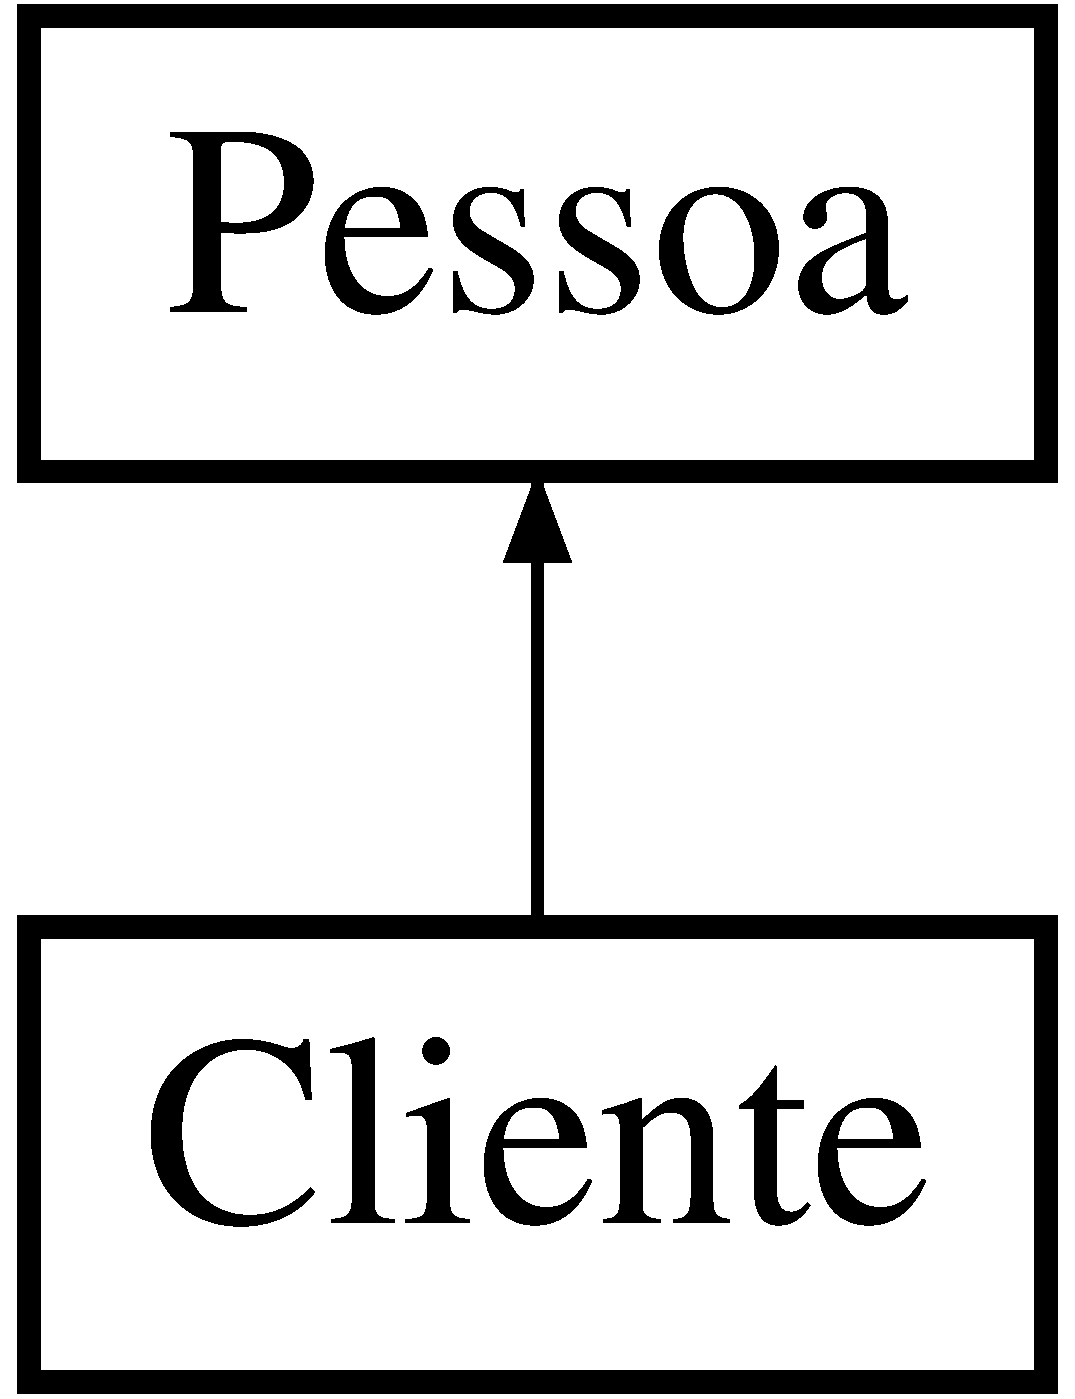
\includegraphics[height=2.000000cm]{class_cliente}
\end{center}
\end{figure}
\subsection*{Public Member Functions}
\begin{DoxyCompactItemize}
\item 
{\bfseries Cliente} (string nome, string cpf, string email, bool socio, string historico)\hypertarget{class_cliente_ae3de50bfea773d769f2741502f3363fd}{}\label{class_cliente_ae3de50bfea773d769f2741502f3363fd}

\item 
{\bfseries Cliente} (int posicao)\hypertarget{class_cliente_ab978791569ca028b959190b5926567bd}{}\label{class_cliente_ab978791569ca028b959190b5926567bd}

\item 
void {\bfseries set\+\_\+socio} (bool socio)\hypertarget{class_cliente_a13f1249779395a989ef94541ce73435b}{}\label{class_cliente_a13f1249779395a989ef94541ce73435b}

\item 
bool {\bfseries get\+\_\+socio} ()\hypertarget{class_cliente_ac19d3bc1957721f87c5605d33d75c020}{}\label{class_cliente_ac19d3bc1957721f87c5605d33d75c020}

\item 
void {\bfseries set\+\_\+historico} (string historico)\hypertarget{class_cliente_ad5192d8b45eced8b09202392c3267c07}{}\label{class_cliente_ad5192d8b45eced8b09202392c3267c07}

\item 
string {\bfseries get\+\_\+historico} ()\hypertarget{class_cliente_a5b6943726dfc79b19d05a9a8b781683e}{}\label{class_cliente_a5b6943726dfc79b19d05a9a8b781683e}

\end{DoxyCompactItemize}


The documentation for this class was generated from the following files\+:\begin{DoxyCompactItemize}
\item 
inc/Cliente.\+hpp\item 
src/Cliente.\+cpp\end{DoxyCompactItemize}

\hypertarget{class_estoque}{}\section{Estoque Class Reference}
\label{class_estoque}\index{Estoque@{Estoque}}
\subsection*{Public Member Functions}
\begin{DoxyCompactItemize}
\item 
virtual void {\bfseries abs} ()=0\hypertarget{class_estoque_ae58fa5f0317c2906e547e8365ec0aaaf}{}\label{class_estoque_ae58fa5f0317c2906e547e8365ec0aaaf}

\end{DoxyCompactItemize}
\subsection*{Static Public Member Functions}
\begin{DoxyCompactItemize}
\item 
static void {\bfseries cadastra\+\_\+produto} ()\hypertarget{class_estoque_a924ac5184642311d4df82cb2bef65391}{}\label{class_estoque_a924ac5184642311d4df82cb2bef65391}

\item 
static void {\bfseries subtrai\+\_\+estoque} (int quant, int posicao)\hypertarget{class_estoque_a2480a2ed74f178c3b08eab98642b81c2}{}\label{class_estoque_a2480a2ed74f178c3b08eab98642b81c2}

\item 
static void {\bfseries adiciona\+\_\+estoque} (int quant, int posicao)\hypertarget{class_estoque_ac23c35a102fc43a0568011657f88df70}{}\label{class_estoque_ac23c35a102fc43a0568011657f88df70}

\item 
static int {\bfseries consulta\+\_\+produto} ()\hypertarget{class_estoque_a8a8e2cf8785baa09afe027f9f938412e}{}\label{class_estoque_a8a8e2cf8785baa09afe027f9f938412e}

\item 
static int {\bfseries consulta\+\_\+produto} (string codigo)\hypertarget{class_estoque_a6352218e6e3a9fbc4a16207bdaa45dc1}{}\label{class_estoque_a6352218e6e3a9fbc4a16207bdaa45dc1}

\item 
static int {\bfseries consulta\+\_\+estoque} (string codigo)\hypertarget{class_estoque_a69db1eed8754357bfb7df9f352e4fcaf}{}\label{class_estoque_a69db1eed8754357bfb7df9f352e4fcaf}

\item 
static void {\bfseries lista\+\_\+produtos} ()\hypertarget{class_estoque_ab538b63ace793abfe0d15eecbb8d4ae0}{}\label{class_estoque_ab538b63ace793abfe0d15eecbb8d4ae0}

\end{DoxyCompactItemize}


The documentation for this class was generated from the following files\+:\begin{DoxyCompactItemize}
\item 
inc/Estoque.\+hpp\item 
src/Estoque.\+cpp\end{DoxyCompactItemize}

\hypertarget{class_loja}{}\section{Loja Class Reference}
\label{class_loja}\index{Loja@{Loja}}
\subsection*{Public Member Functions}
\begin{DoxyCompactItemize}
\item 
virtual int {\bfseries abs} ()=0\hypertarget{class_loja_a891ad86180f9bdc3b2d97592b51d36a2}{}\label{class_loja_a891ad86180f9bdc3b2d97592b51d36a2}

\end{DoxyCompactItemize}
\subsection*{Static Public Member Functions}
\begin{DoxyCompactItemize}
\item 
static void {\bfseries modo\+\_\+venda} ()\hypertarget{class_loja_a5e9ae50837083855335d4f9dd58d7615}{}\label{class_loja_a5e9ae50837083855335d4f9dd58d7615}

\item 
static void {\bfseries modo\+\_\+estoque} ()\hypertarget{class_loja_a6480b80d0a09a532267d8f388d866005}{}\label{class_loja_a6480b80d0a09a532267d8f388d866005}

\item 
static void {\bfseries modo\+\_\+recomendacao} ()\hypertarget{class_loja_a468423ff1ac93d7a65d24f52eafe2276}{}\label{class_loja_a468423ff1ac93d7a65d24f52eafe2276}

\item 
static void {\bfseries cadastra\+\_\+cliente} ()\hypertarget{class_loja_a046efae41cdbf838169aaa1773249842}{}\label{class_loja_a046efae41cdbf838169aaa1773249842}

\item 
static bool {\bfseries consulta\+\_\+socio} (string cpf)\hypertarget{class_loja_a1b6910218ccb9274dcbb6635fdb562f8}{}\label{class_loja_a1b6910218ccb9274dcbb6635fdb562f8}

\item 
static int {\bfseries consulta\+\_\+cliente} (string cpf)\hypertarget{class_loja_af77ca2356affc8acc06abaac4ce72962}{}\label{class_loja_af77ca2356affc8acc06abaac4ce72962}

\item 
static void {\bfseries cupom\+\_\+fiscal} (string nome, string cpf, float preco)\hypertarget{class_loja_aa6792e6f3f268652266275fc0d096fab}{}\label{class_loja_aa6792e6f3f268652266275fc0d096fab}

\item 
static void {\bfseries modo\+\_\+balanco} ()\hypertarget{class_loja_a483d73b9661da5d7ce556ddde427e3f7}{}\label{class_loja_a483d73b9661da5d7ce556ddde427e3f7}

\end{DoxyCompactItemize}


The documentation for this class was generated from the following files\+:\begin{DoxyCompactItemize}
\item 
inc/Loja.\+hpp\item 
src/Loja.\+cpp\end{DoxyCompactItemize}

\hypertarget{class_pessoa}{}\section{Pessoa Class Reference}
\label{class_pessoa}\index{Pessoa@{Pessoa}}
Inheritance diagram for Pessoa\+:\begin{figure}[H]
\begin{center}
\leavevmode
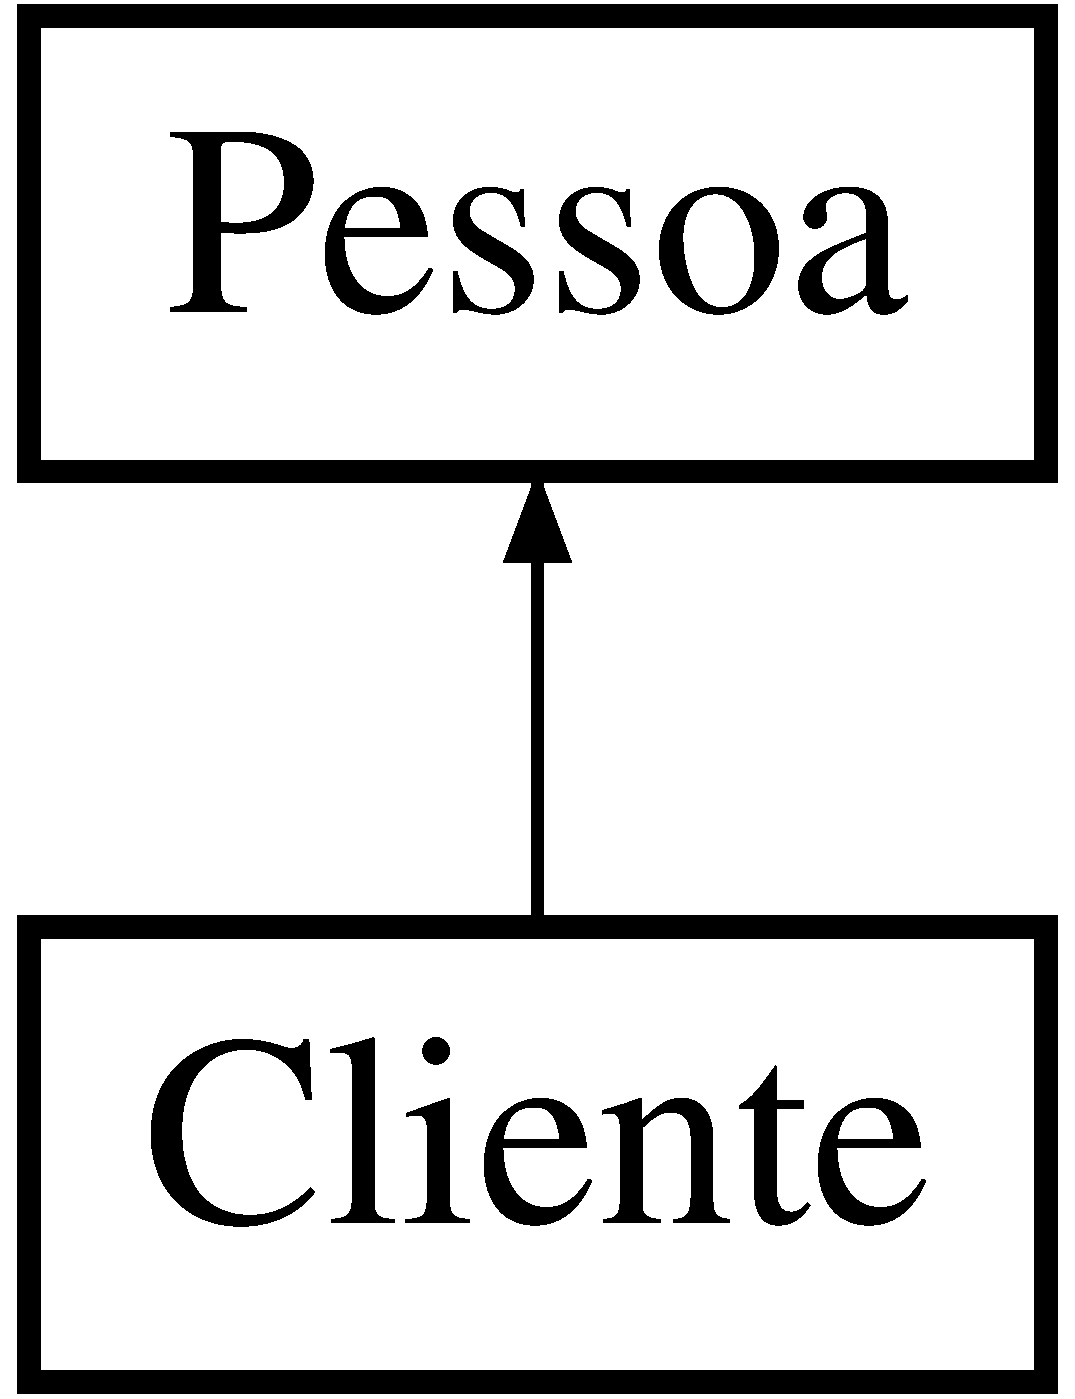
\includegraphics[height=2.000000cm]{class_pessoa}
\end{center}
\end{figure}
\subsection*{Public Member Functions}
\begin{DoxyCompactItemize}
\item 
void {\bfseries set\+\_\+nome} (string nome)\hypertarget{class_pessoa_ade7bf4832051a8b35b2531632c986b7a}{}\label{class_pessoa_ade7bf4832051a8b35b2531632c986b7a}

\item 
string {\bfseries get\+\_\+nome} ()\hypertarget{class_pessoa_a7fc758a1ba17e56d95dfbbc1e65cbedf}{}\label{class_pessoa_a7fc758a1ba17e56d95dfbbc1e65cbedf}

\item 
void {\bfseries set\+\_\+cpf} (string cpf)\hypertarget{class_pessoa_ae7fa0ed8427a1674ac87efd327aa2009}{}\label{class_pessoa_ae7fa0ed8427a1674ac87efd327aa2009}

\item 
string {\bfseries get\+\_\+cpf} ()\hypertarget{class_pessoa_a95123b811bca5c1d4c72233b29f227dd}{}\label{class_pessoa_a95123b811bca5c1d4c72233b29f227dd}

\item 
void {\bfseries set\+\_\+email} (string email)\hypertarget{class_pessoa_a829da31a467d19d469925370301c34bd}{}\label{class_pessoa_a829da31a467d19d469925370301c34bd}

\item 
string {\bfseries get\+\_\+email} ()\hypertarget{class_pessoa_afc904106ca6695d07a382a0300f033ba}{}\label{class_pessoa_afc904106ca6695d07a382a0300f033ba}

\end{DoxyCompactItemize}


The documentation for this class was generated from the following files\+:\begin{DoxyCompactItemize}
\item 
inc/Pessoa.\+hpp\item 
src/Pessoa.\+cpp\end{DoxyCompactItemize}

\hypertarget{class_produto}{}\section{Produto Class Reference}
\label{class_produto}\index{Produto@{Produto}}
\subsection*{Public Member Functions}
\begin{DoxyCompactItemize}
\item 
{\bfseries Produto} (string codigo, string nome, string categoria, string preco, string quantidade)\hypertarget{class_produto_a513cd996c33046f28ce973f61c68ea7e}{}\label{class_produto_a513cd996c33046f28ce973f61c68ea7e}

\item 
void {\bfseries set\+\_\+codigo} (string codigo)\hypertarget{class_produto_ab6816364c76995c529bdbb1d3d6999ac}{}\label{class_produto_ab6816364c76995c529bdbb1d3d6999ac}

\item 
string {\bfseries get\+\_\+codigo} ()\hypertarget{class_produto_a5fee389ee57a450e988a6ebc9e6db157}{}\label{class_produto_a5fee389ee57a450e988a6ebc9e6db157}

\item 
void {\bfseries set\+\_\+nome} (string nome)\hypertarget{class_produto_a55230e3937d26a09b2a143a2c2d5173d}{}\label{class_produto_a55230e3937d26a09b2a143a2c2d5173d}

\item 
string {\bfseries get\+\_\+nome} ()\hypertarget{class_produto_af3226ae7eafdec16f13f266464be7596}{}\label{class_produto_af3226ae7eafdec16f13f266464be7596}

\item 
void {\bfseries set\+\_\+categoria} (string categoria)\hypertarget{class_produto_a10b0890a8448b51ac46d8c2bc461d3d8}{}\label{class_produto_a10b0890a8448b51ac46d8c2bc461d3d8}

\item 
string {\bfseries get\+\_\+categoria} ()\hypertarget{class_produto_a4983d87d5c8672a7d867d063e1d1755e}{}\label{class_produto_a4983d87d5c8672a7d867d063e1d1755e}

\item 
void {\bfseries set\+\_\+quantidade} (string quantidade)\hypertarget{class_produto_a2bc9a6c48b870d99bc16da38fb738a36}{}\label{class_produto_a2bc9a6c48b870d99bc16da38fb738a36}

\item 
string {\bfseries get\+\_\+quantidade} ()\hypertarget{class_produto_a5139aab83ed7e79e80a50b3f0099e072}{}\label{class_produto_a5139aab83ed7e79e80a50b3f0099e072}

\item 
void {\bfseries set\+\_\+preco} (string preco)\hypertarget{class_produto_a5e71ed00267a2b4b8617ccf1c06ab258}{}\label{class_produto_a5e71ed00267a2b4b8617ccf1c06ab258}

\item 
string {\bfseries get\+\_\+preco} ()\hypertarget{class_produto_ad531cb3d2629b04e8fca7e9a4d72fb88}{}\label{class_produto_ad531cb3d2629b04e8fca7e9a4d72fb88}

\end{DoxyCompactItemize}


The documentation for this class was generated from the following files\+:\begin{DoxyCompactItemize}
\item 
inc/Produto.\+hpp\item 
src/Produto.\+cpp\end{DoxyCompactItemize}

%--- End generated contents ---

% Index
\backmatter
\newpage
\phantomsection
\clearemptydoublepage
\addcontentsline{toc}{chapter}{Index}
\printindex

\end{document}
